\chapter{Results}
\label{chapterlabel6}

One case from the permutations of the simulations is being used as the control model. The case was taken based on most common assumptions in the current research, which is the case of a normal aorta, smoothened wall and with Newtonian fluid. The mesh selected was the mesh 3 ($\sim$600,000 elements) \cite{Steinman2012AssumptionsHemodynamics}.

\section{Outlet flow and pressure comparison}
A comparison of the outlet conditions were compared. The results were compared by calculating the mean absolute percentage error (MAPE) between control model and the model with modified conditions:

\begin{align}
    MAPE = \frac{y_{i}-y_{control}}{y_{control}} \times 100 \%
\end{align}

where y is the parameter of interest which in the comparison is either the flow rate or the pressure. \par
A comparison of the outlet pressure and flow can be seen on the Figures \ref{fig:flow} and \ref{fig:pressure}. A comparison with the control simulation shows that the pressure at the outlets are very similar across the models as the mean absolute percentage error is less then 1\% (as seen in the Table \ref{tab:pererr}). However significant differences can be seen in the flow curves where depending on the model assumptions taken into account. On the Table \ref{tab:pererr}, it can be seen that very little differences can be seen when the viscosity model is modified while the smoothening of the aortic geometry yields very high mean percentage error. \par
\begin{figure}
     \centering
     \begin{subfigure}[b]{0.49\textwidth}
         \centering
         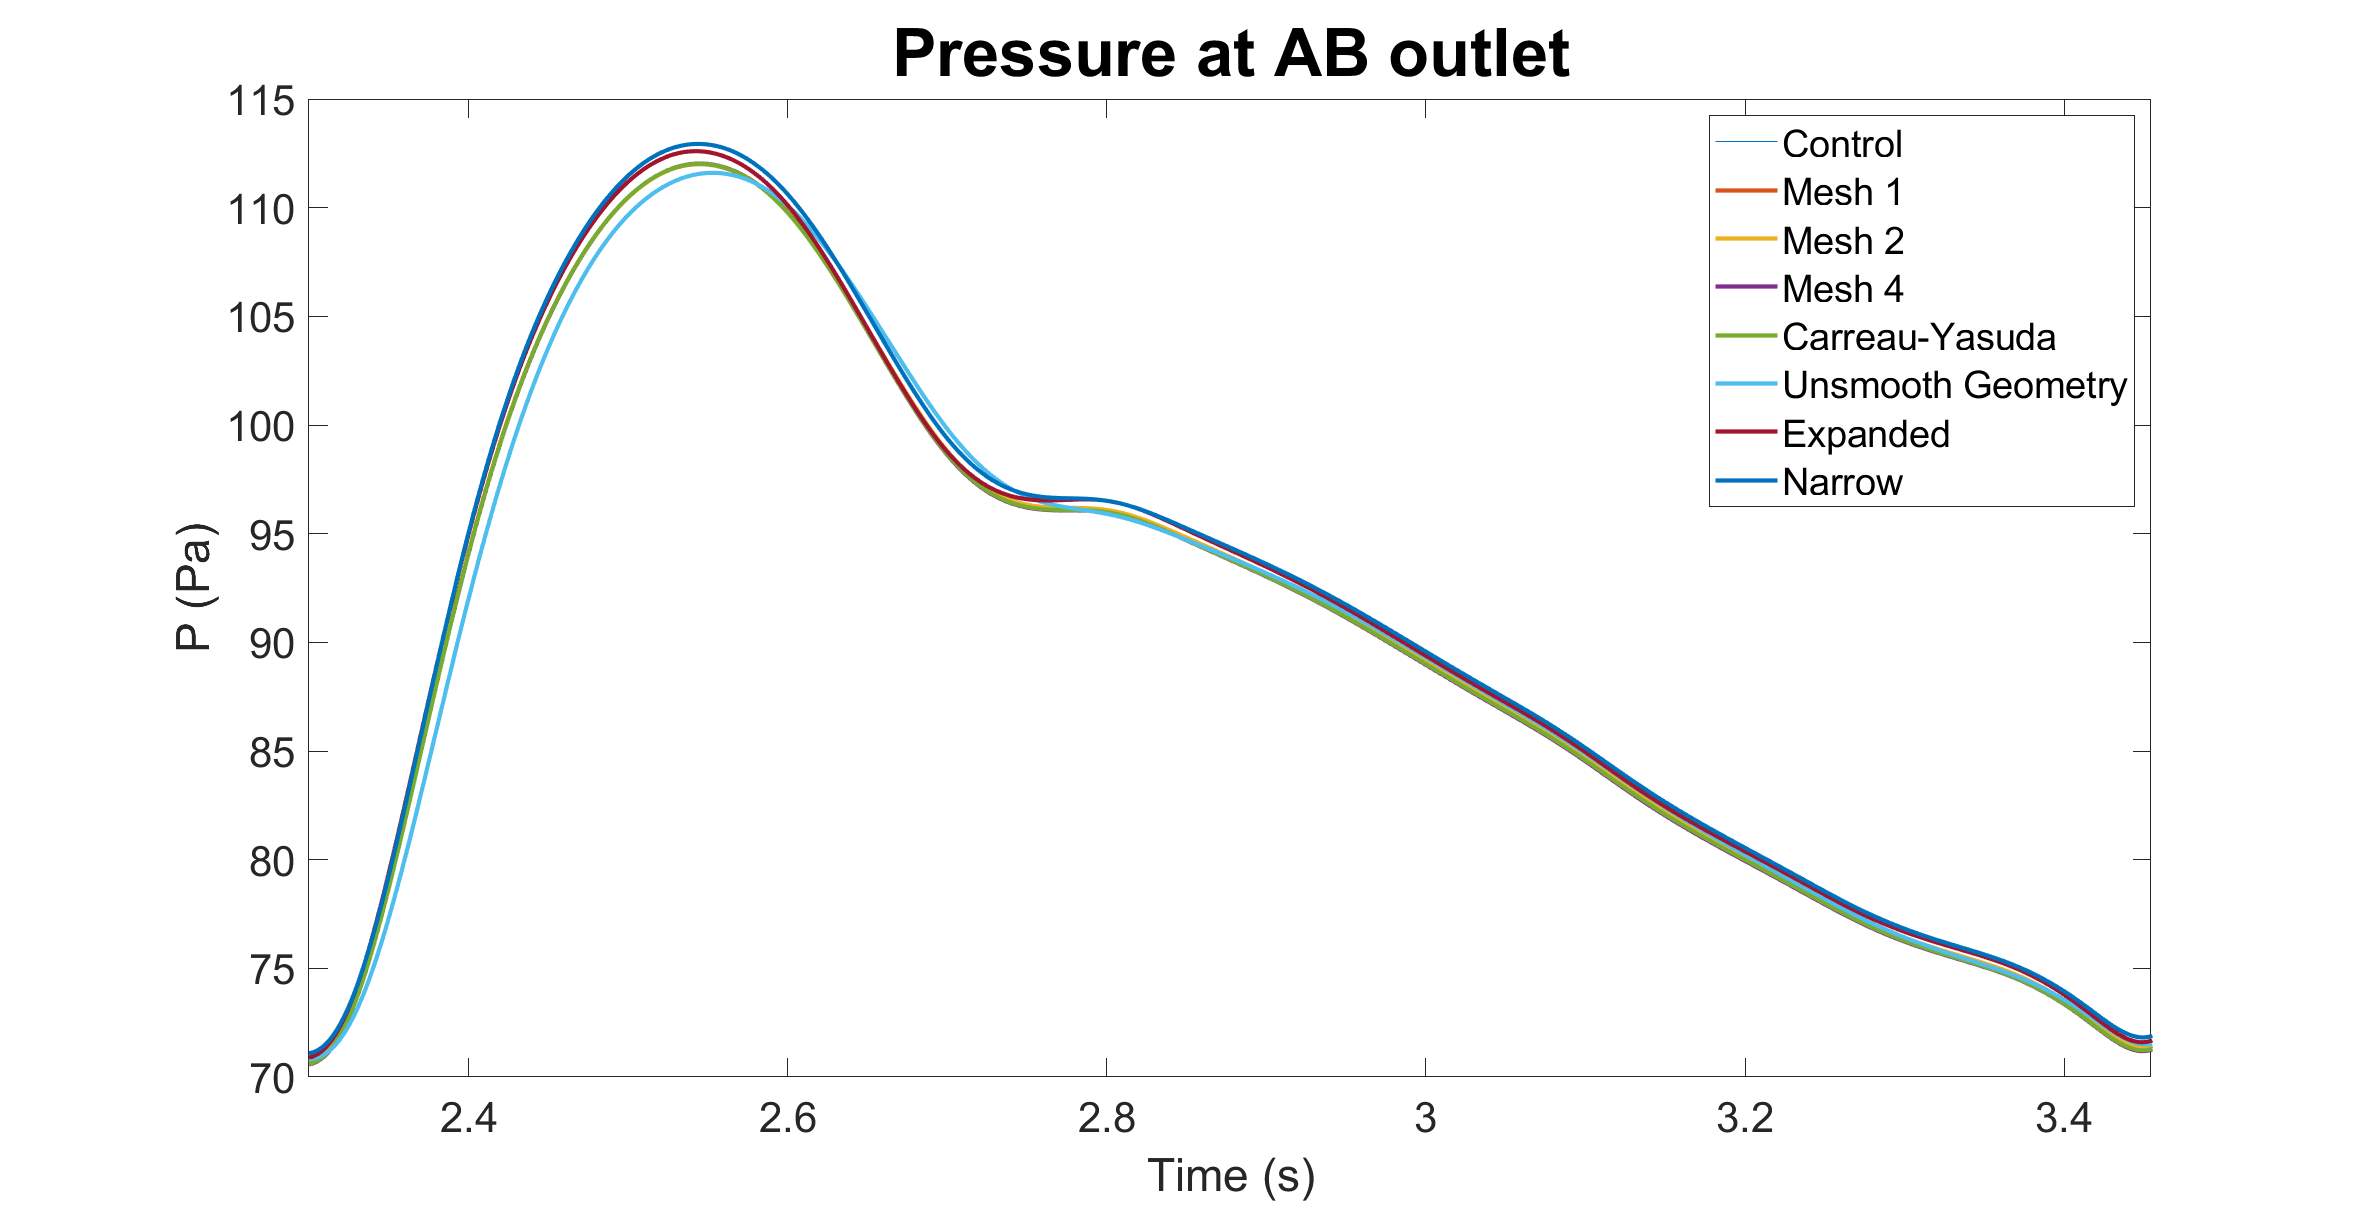
\includegraphics[width=\textwidth]{Figures/PAB.png}
     \end{subfigure}
     \hfill
     \begin{subfigure}[b]{0.49\textwidth}
         \centering
         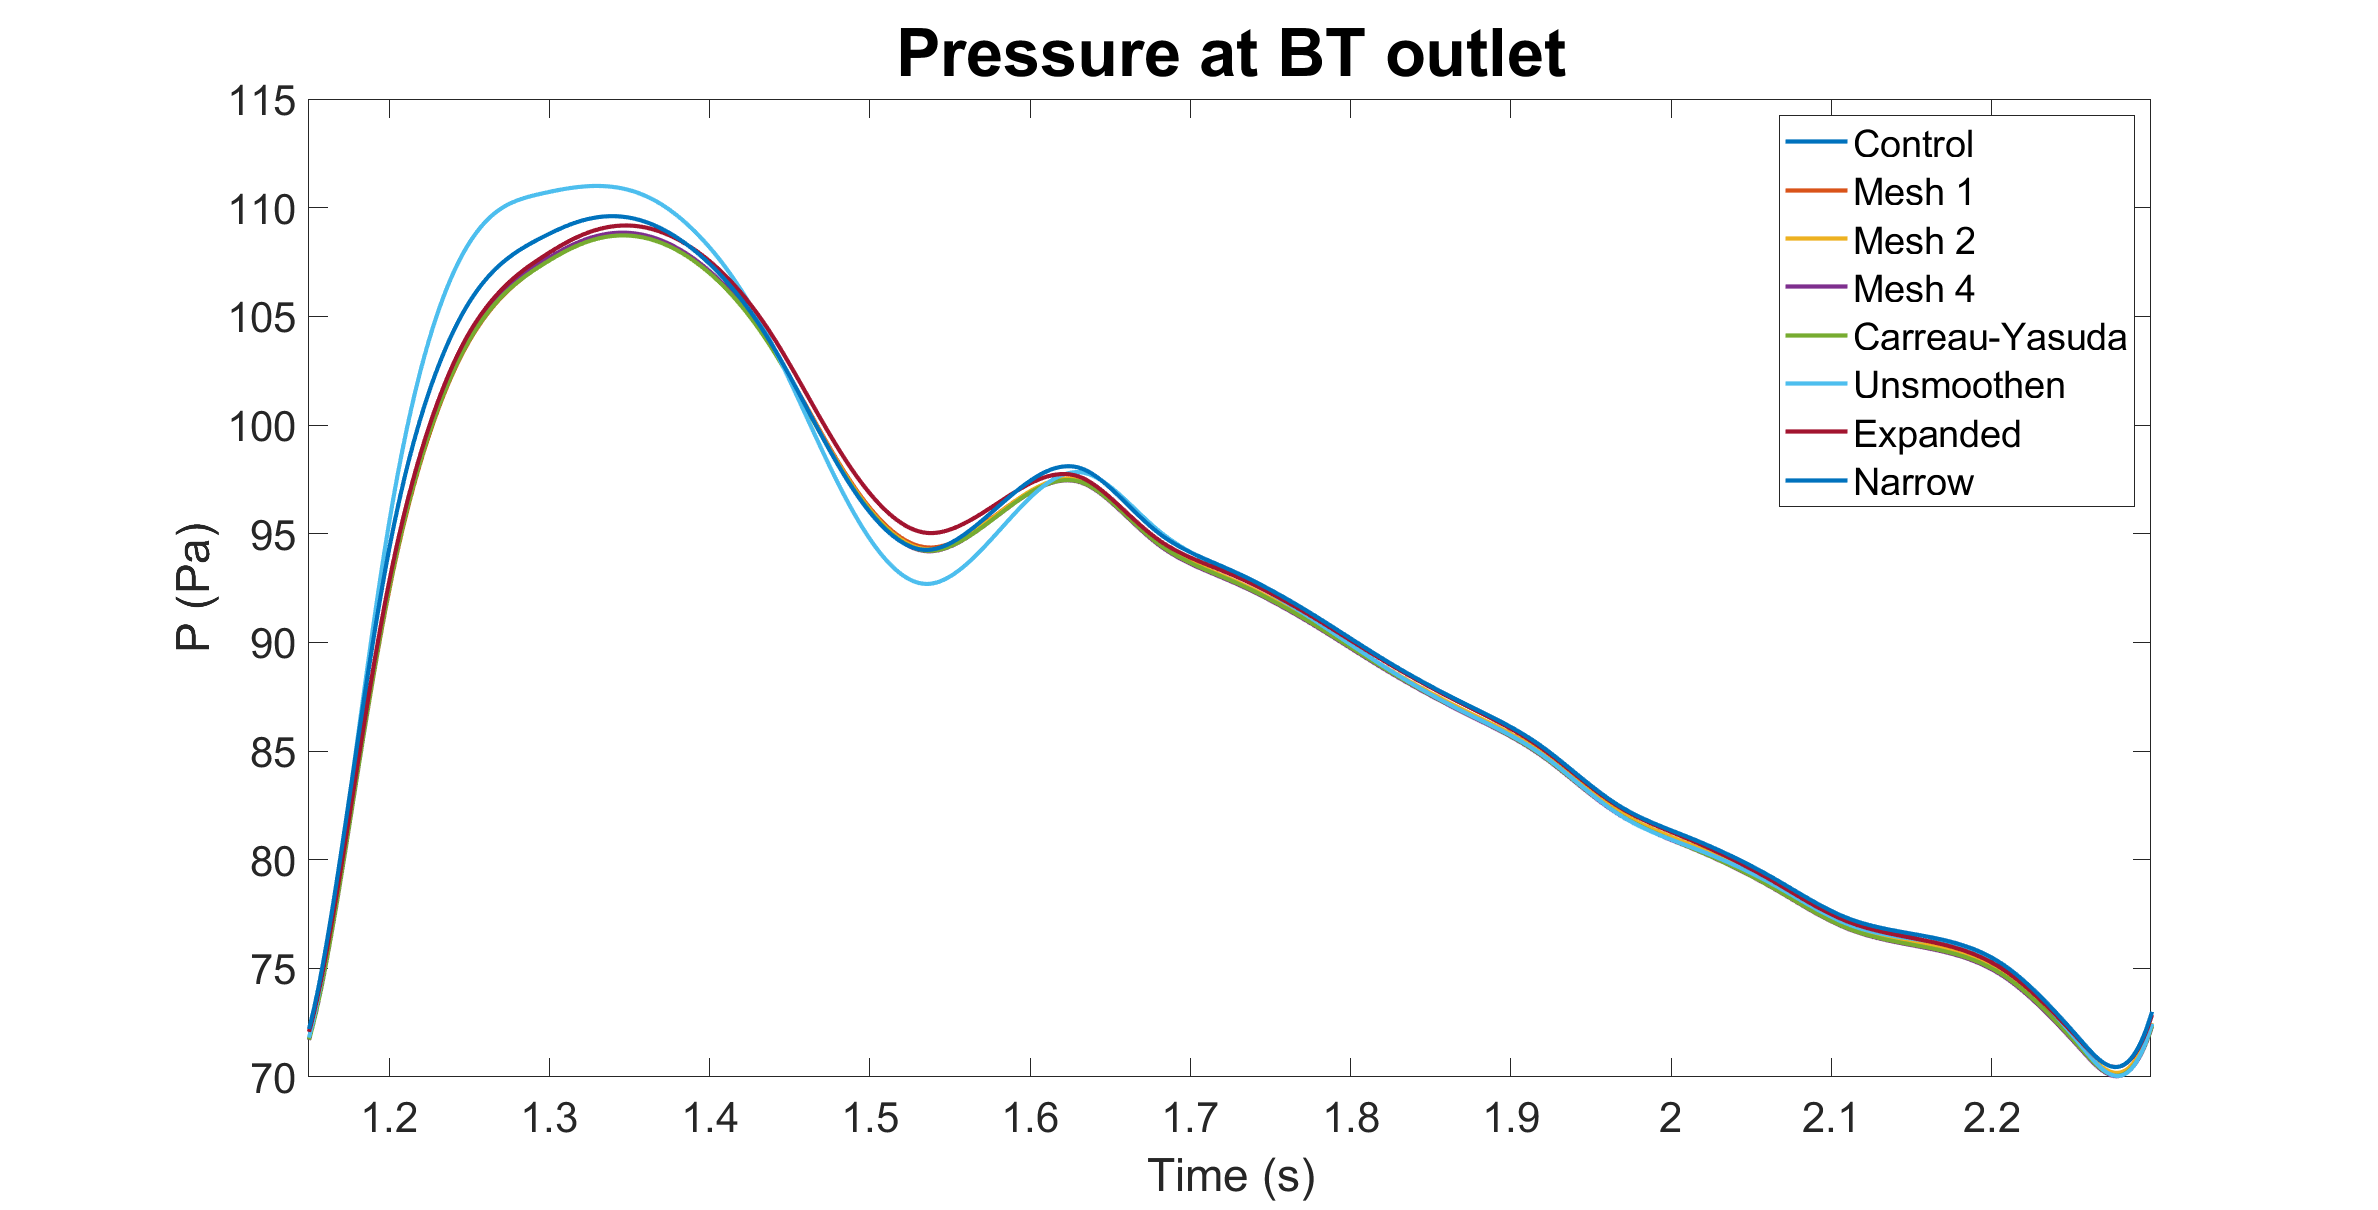
\includegraphics[width=\textwidth]{Figures/PBT.png}
     \end{subfigure}
     \hfill
     \begin{subfigure}[b]{0.49\textwidth}
         \centering
         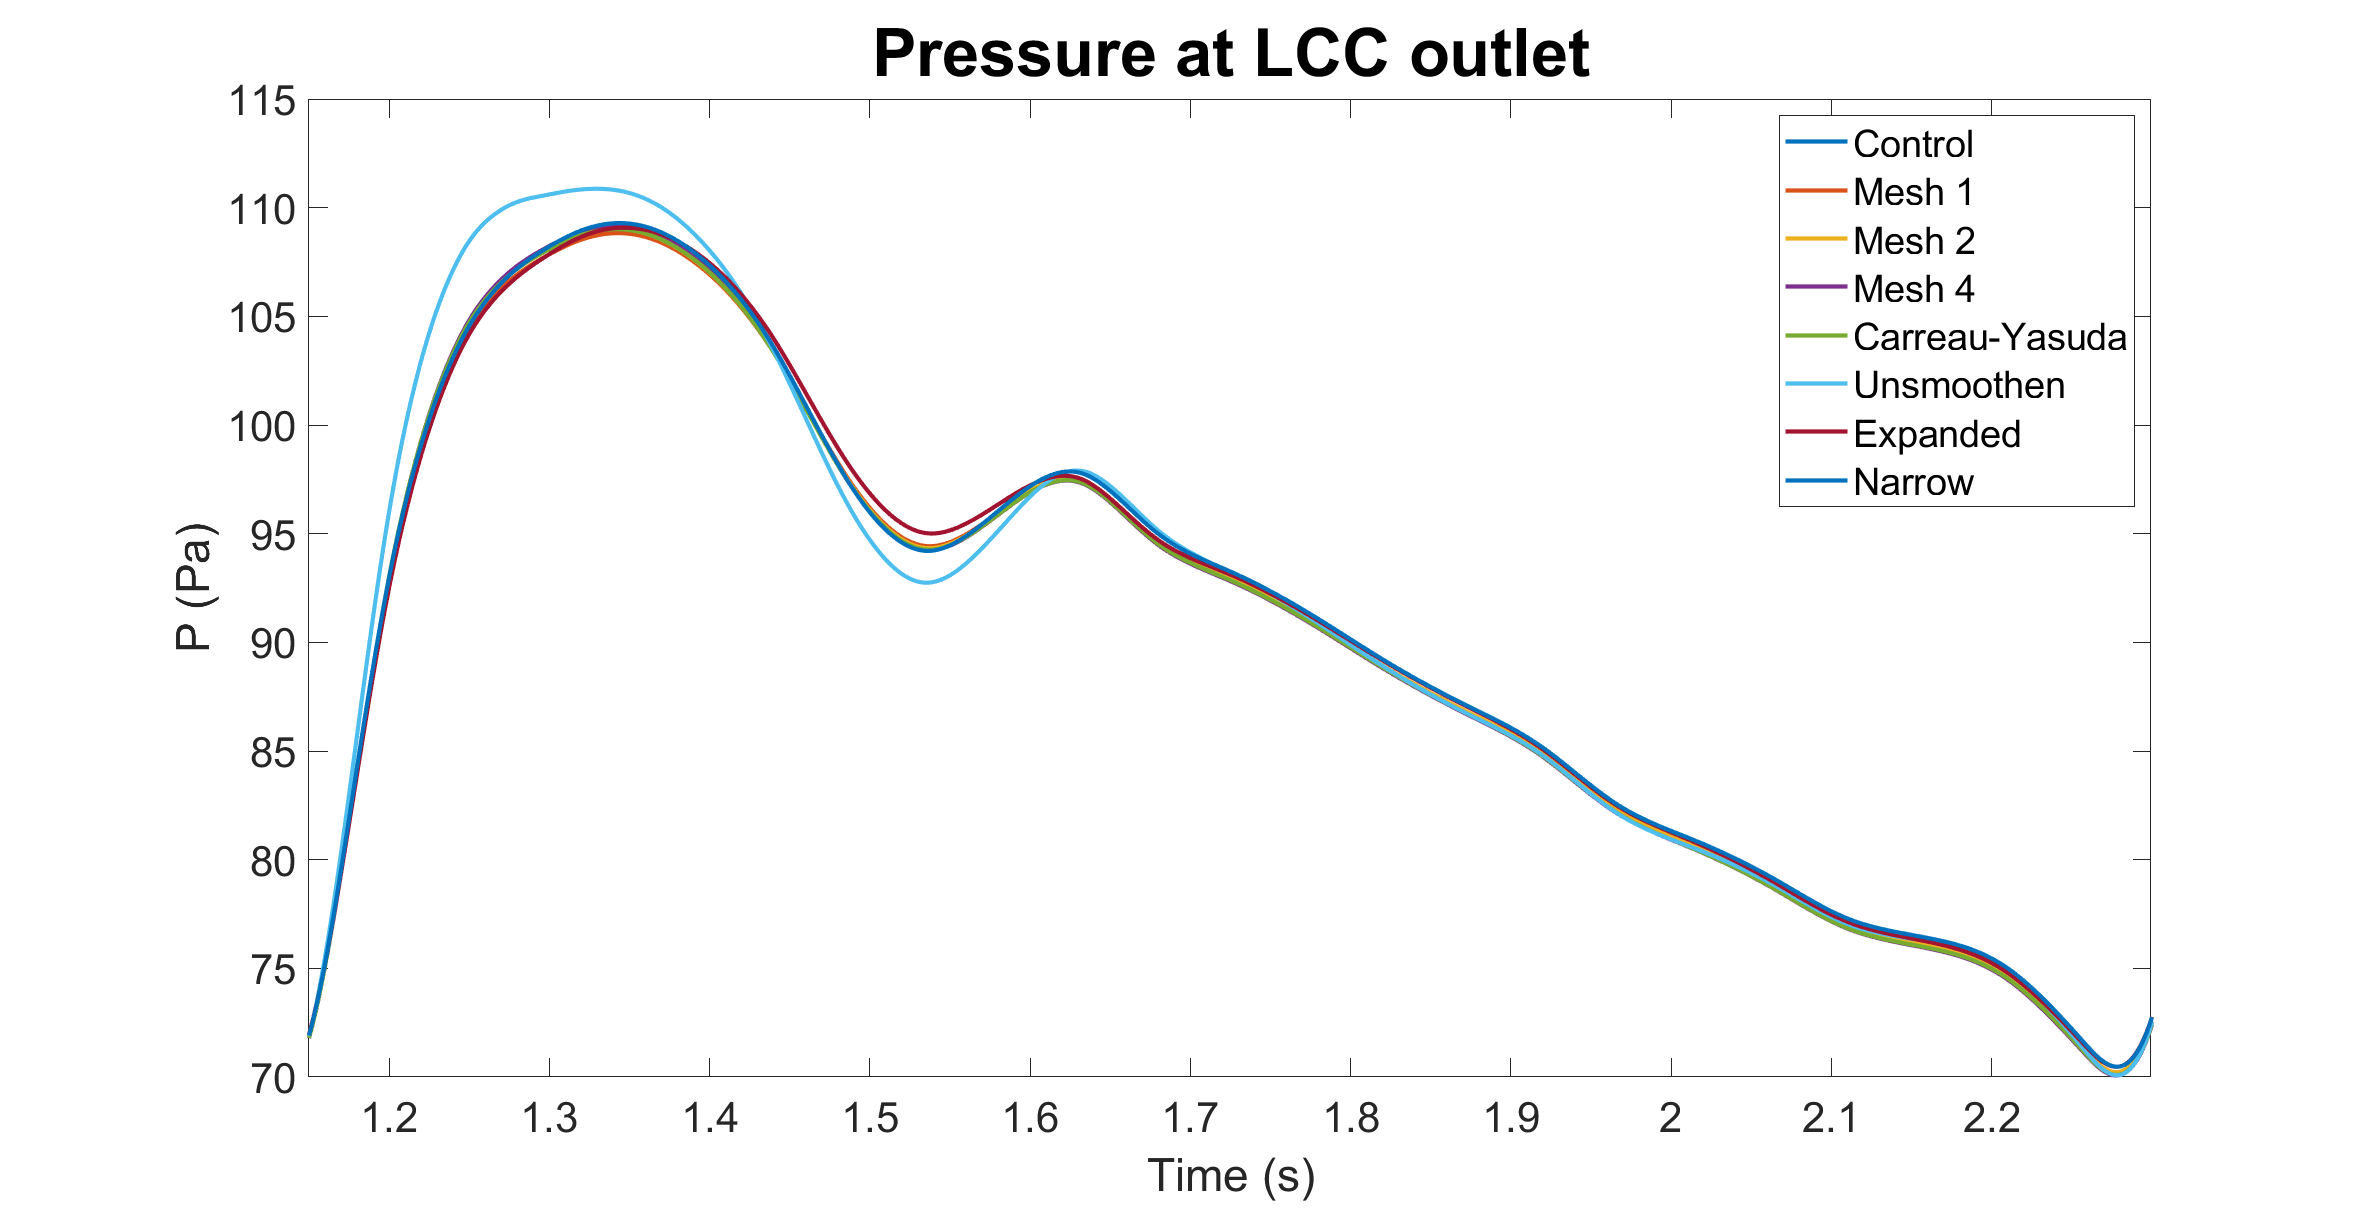
\includegraphics[width=\textwidth]{Figures/PLCC.png}
     \end{subfigure}
     \hfill
     \begin{subfigure}[b]{0.49\textwidth}
         \centering
         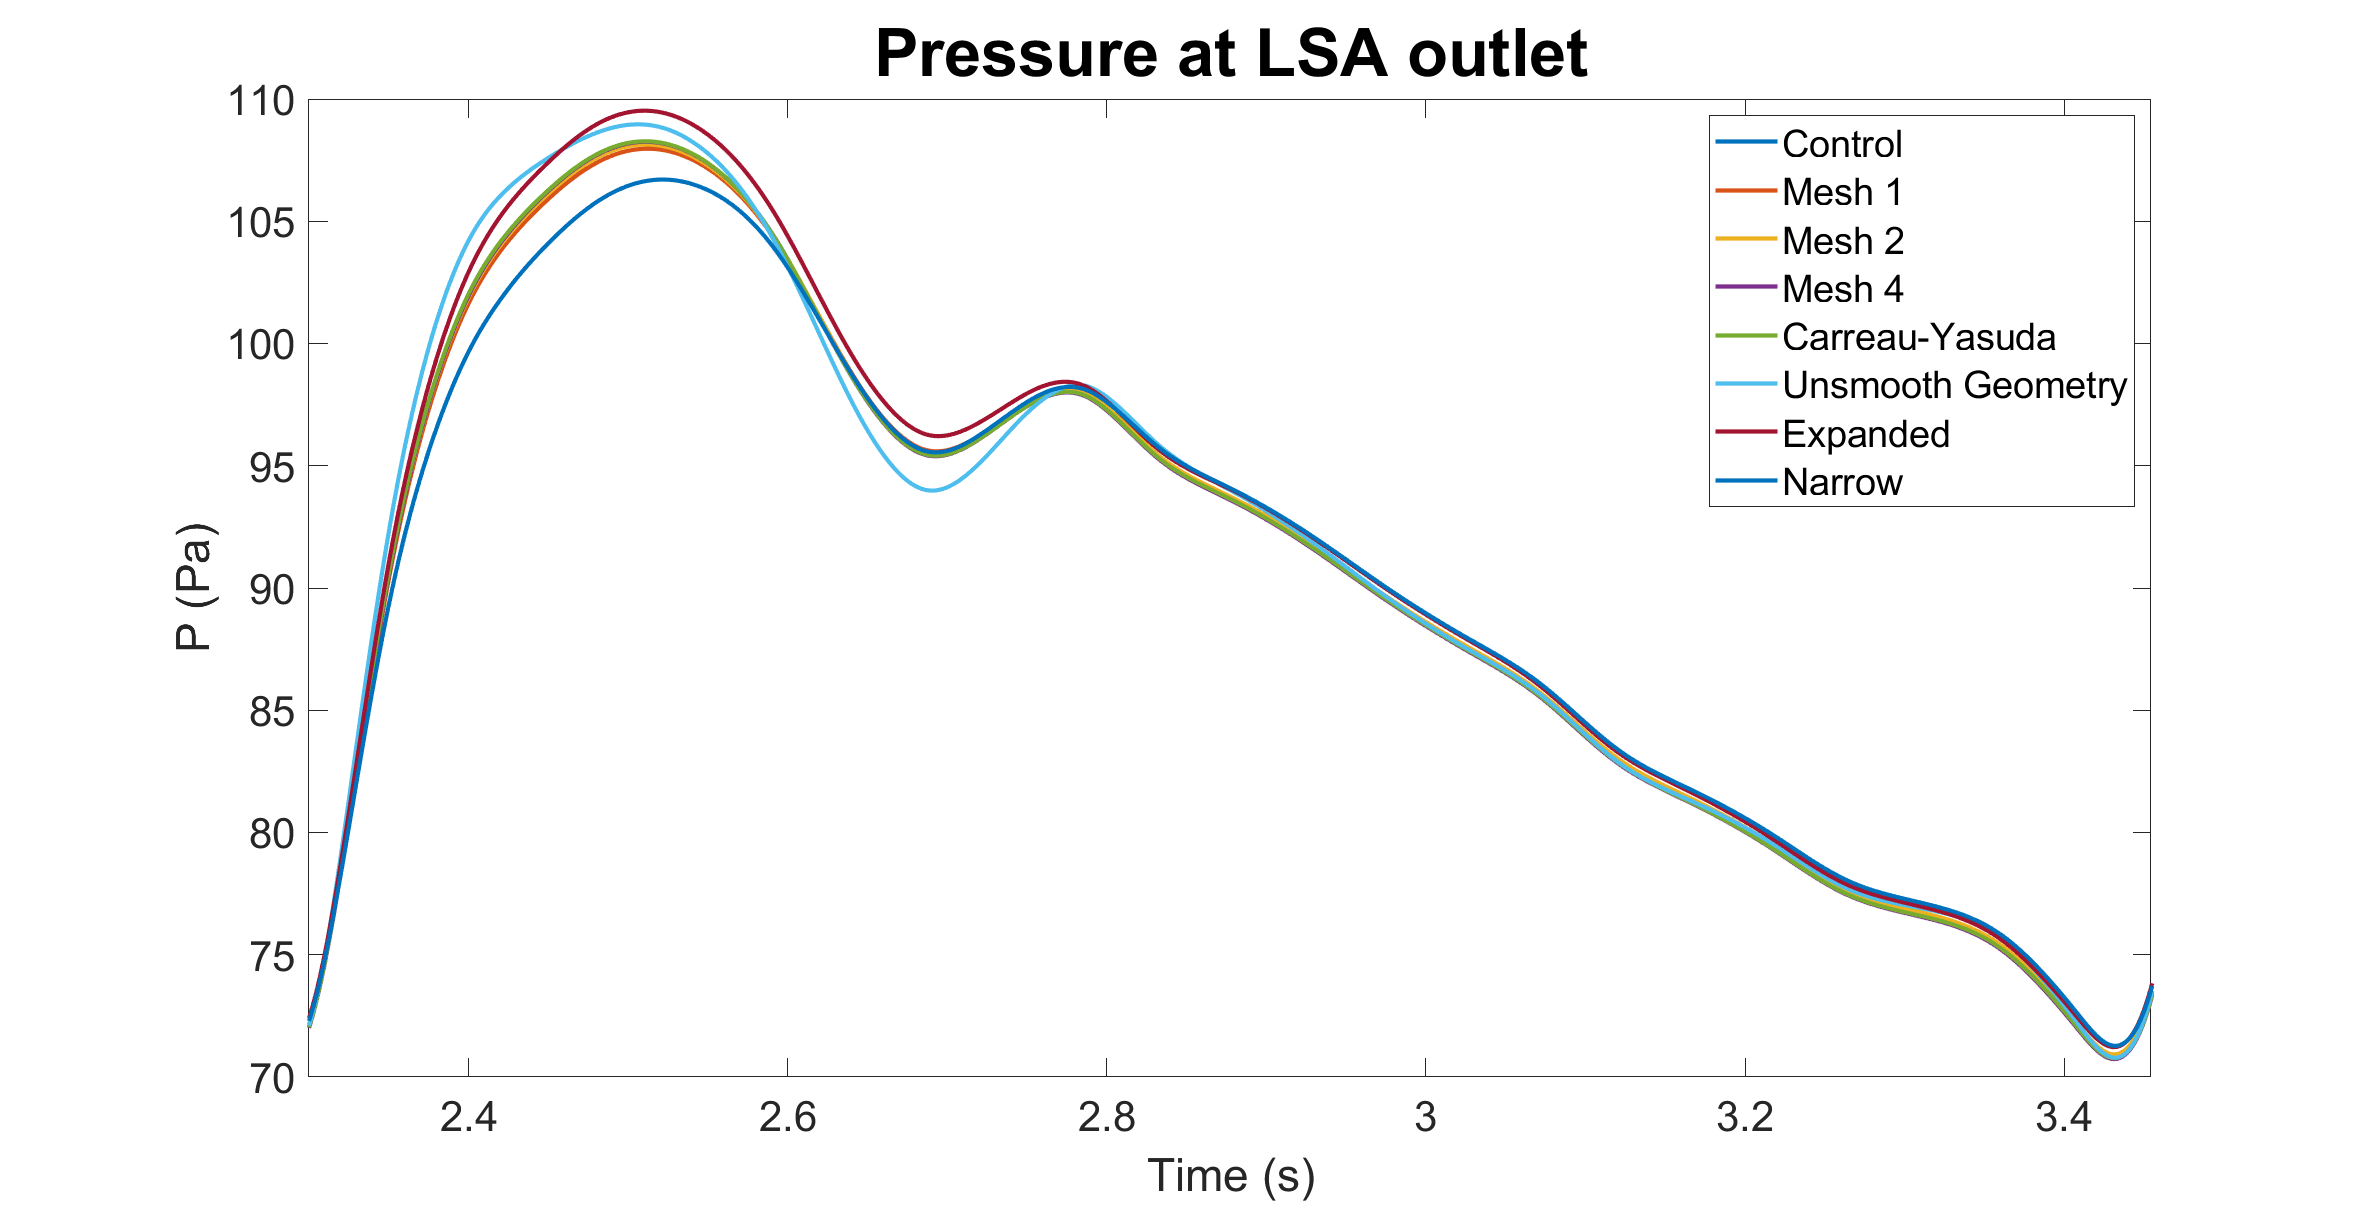
\includegraphics[width=\textwidth]{Figures/PLSA.png}
     \end{subfigure}
        \caption{The pressure at the different outlets}
        \label{fig:pressure}
\end{figure}

\begin{figure}
     \centering
     \begin{subfigure}[b]{0.49\textwidth}
         \centering
         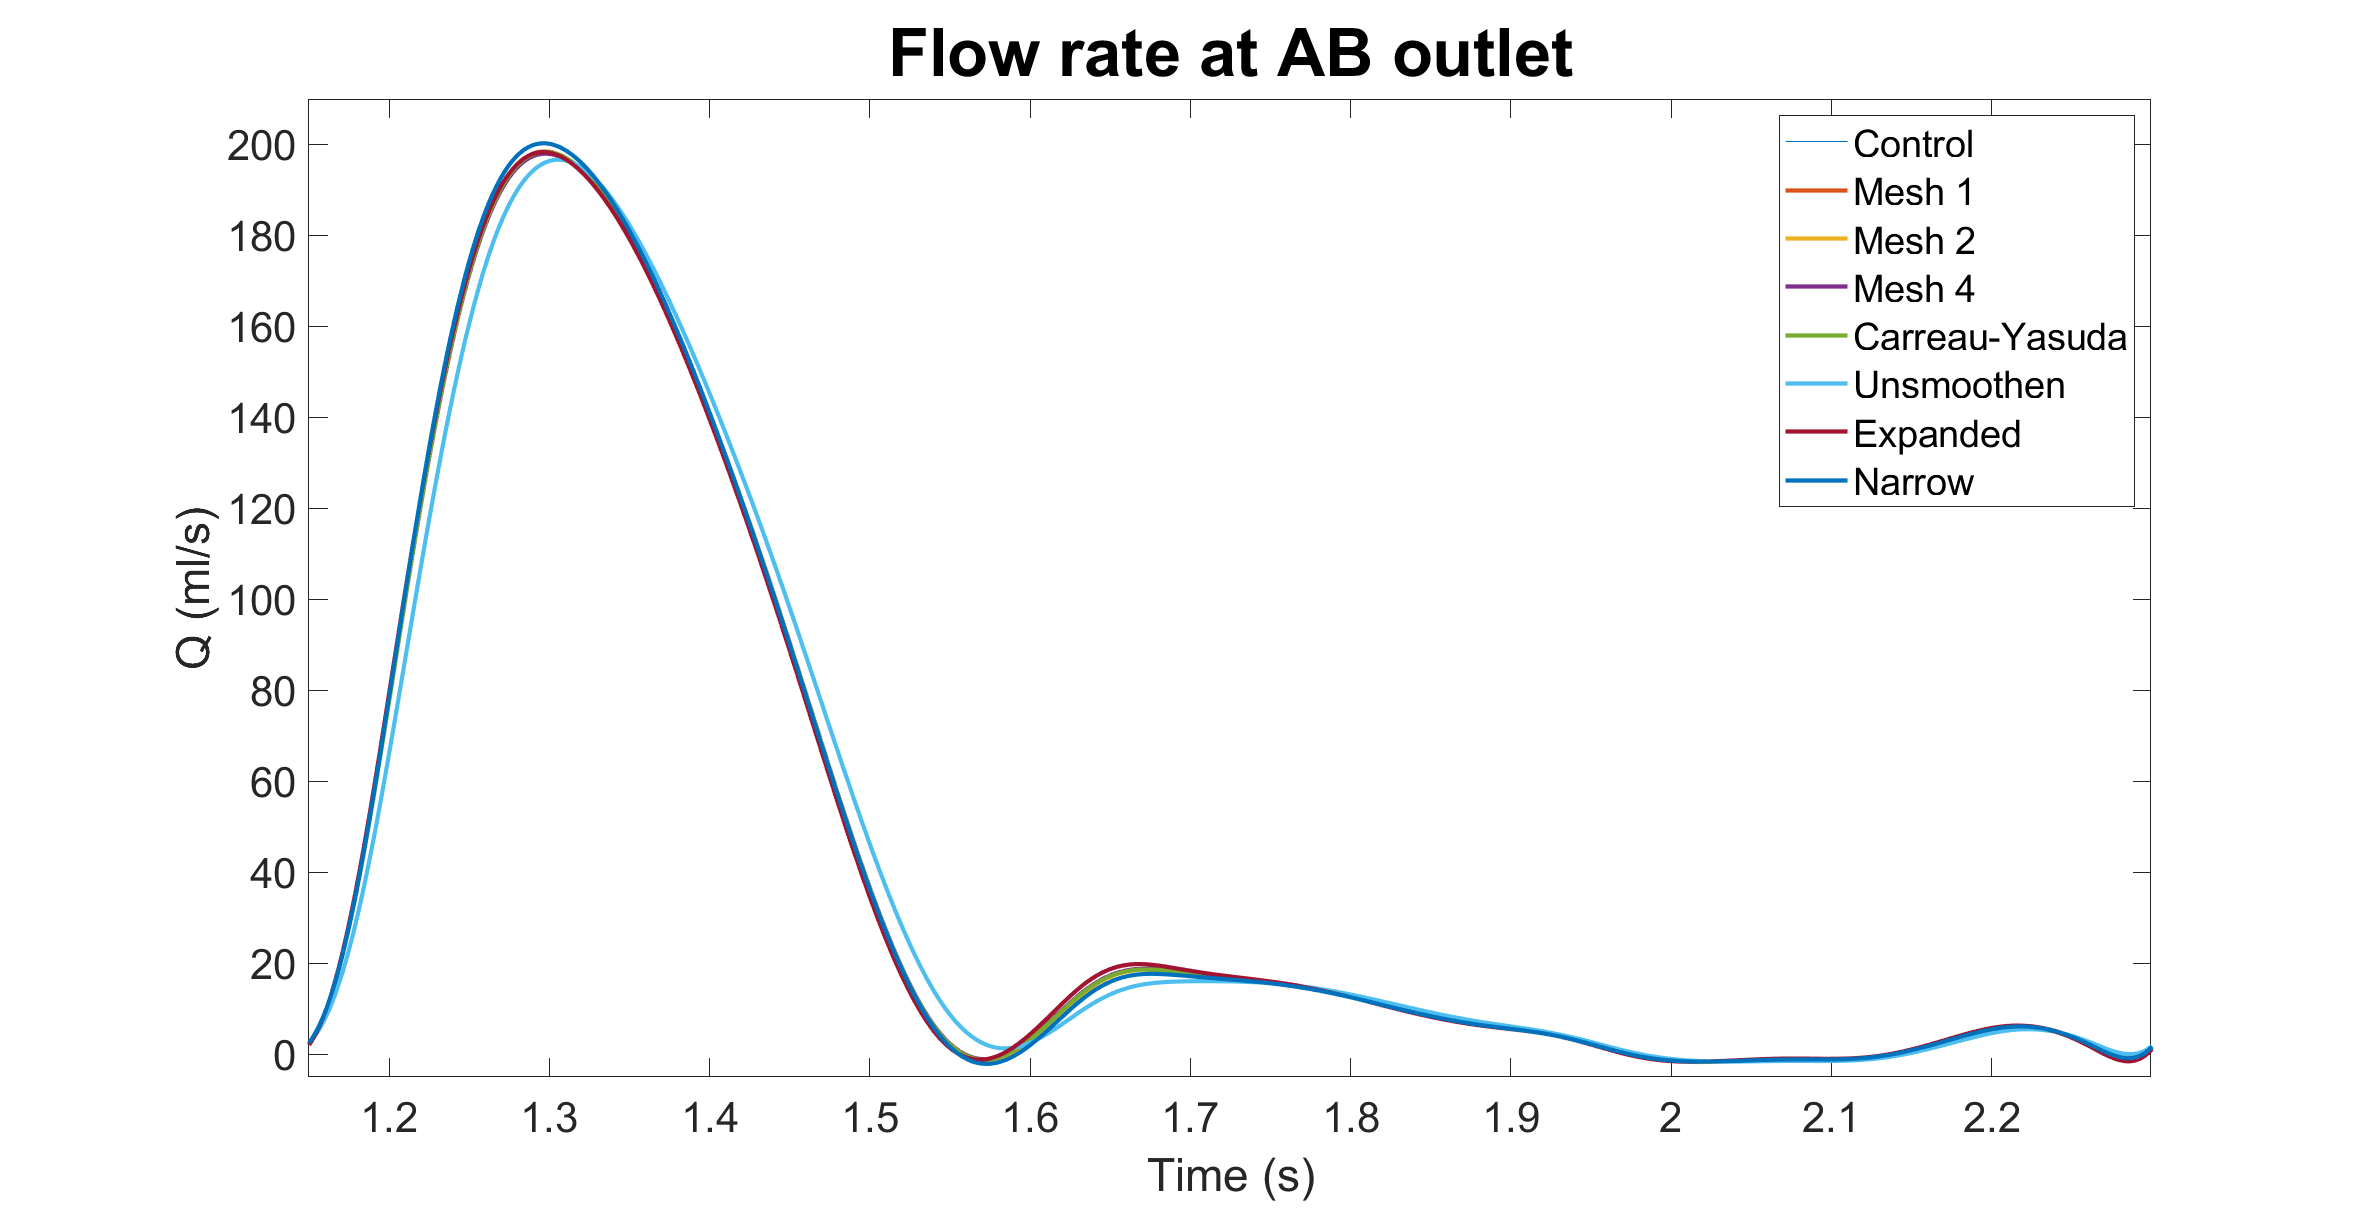
\includegraphics[width=\textwidth]{Figures/QAB.png}
     \end{subfigure}
     \hfill
     \begin{subfigure}[b]{0.49\textwidth}
         \centering
         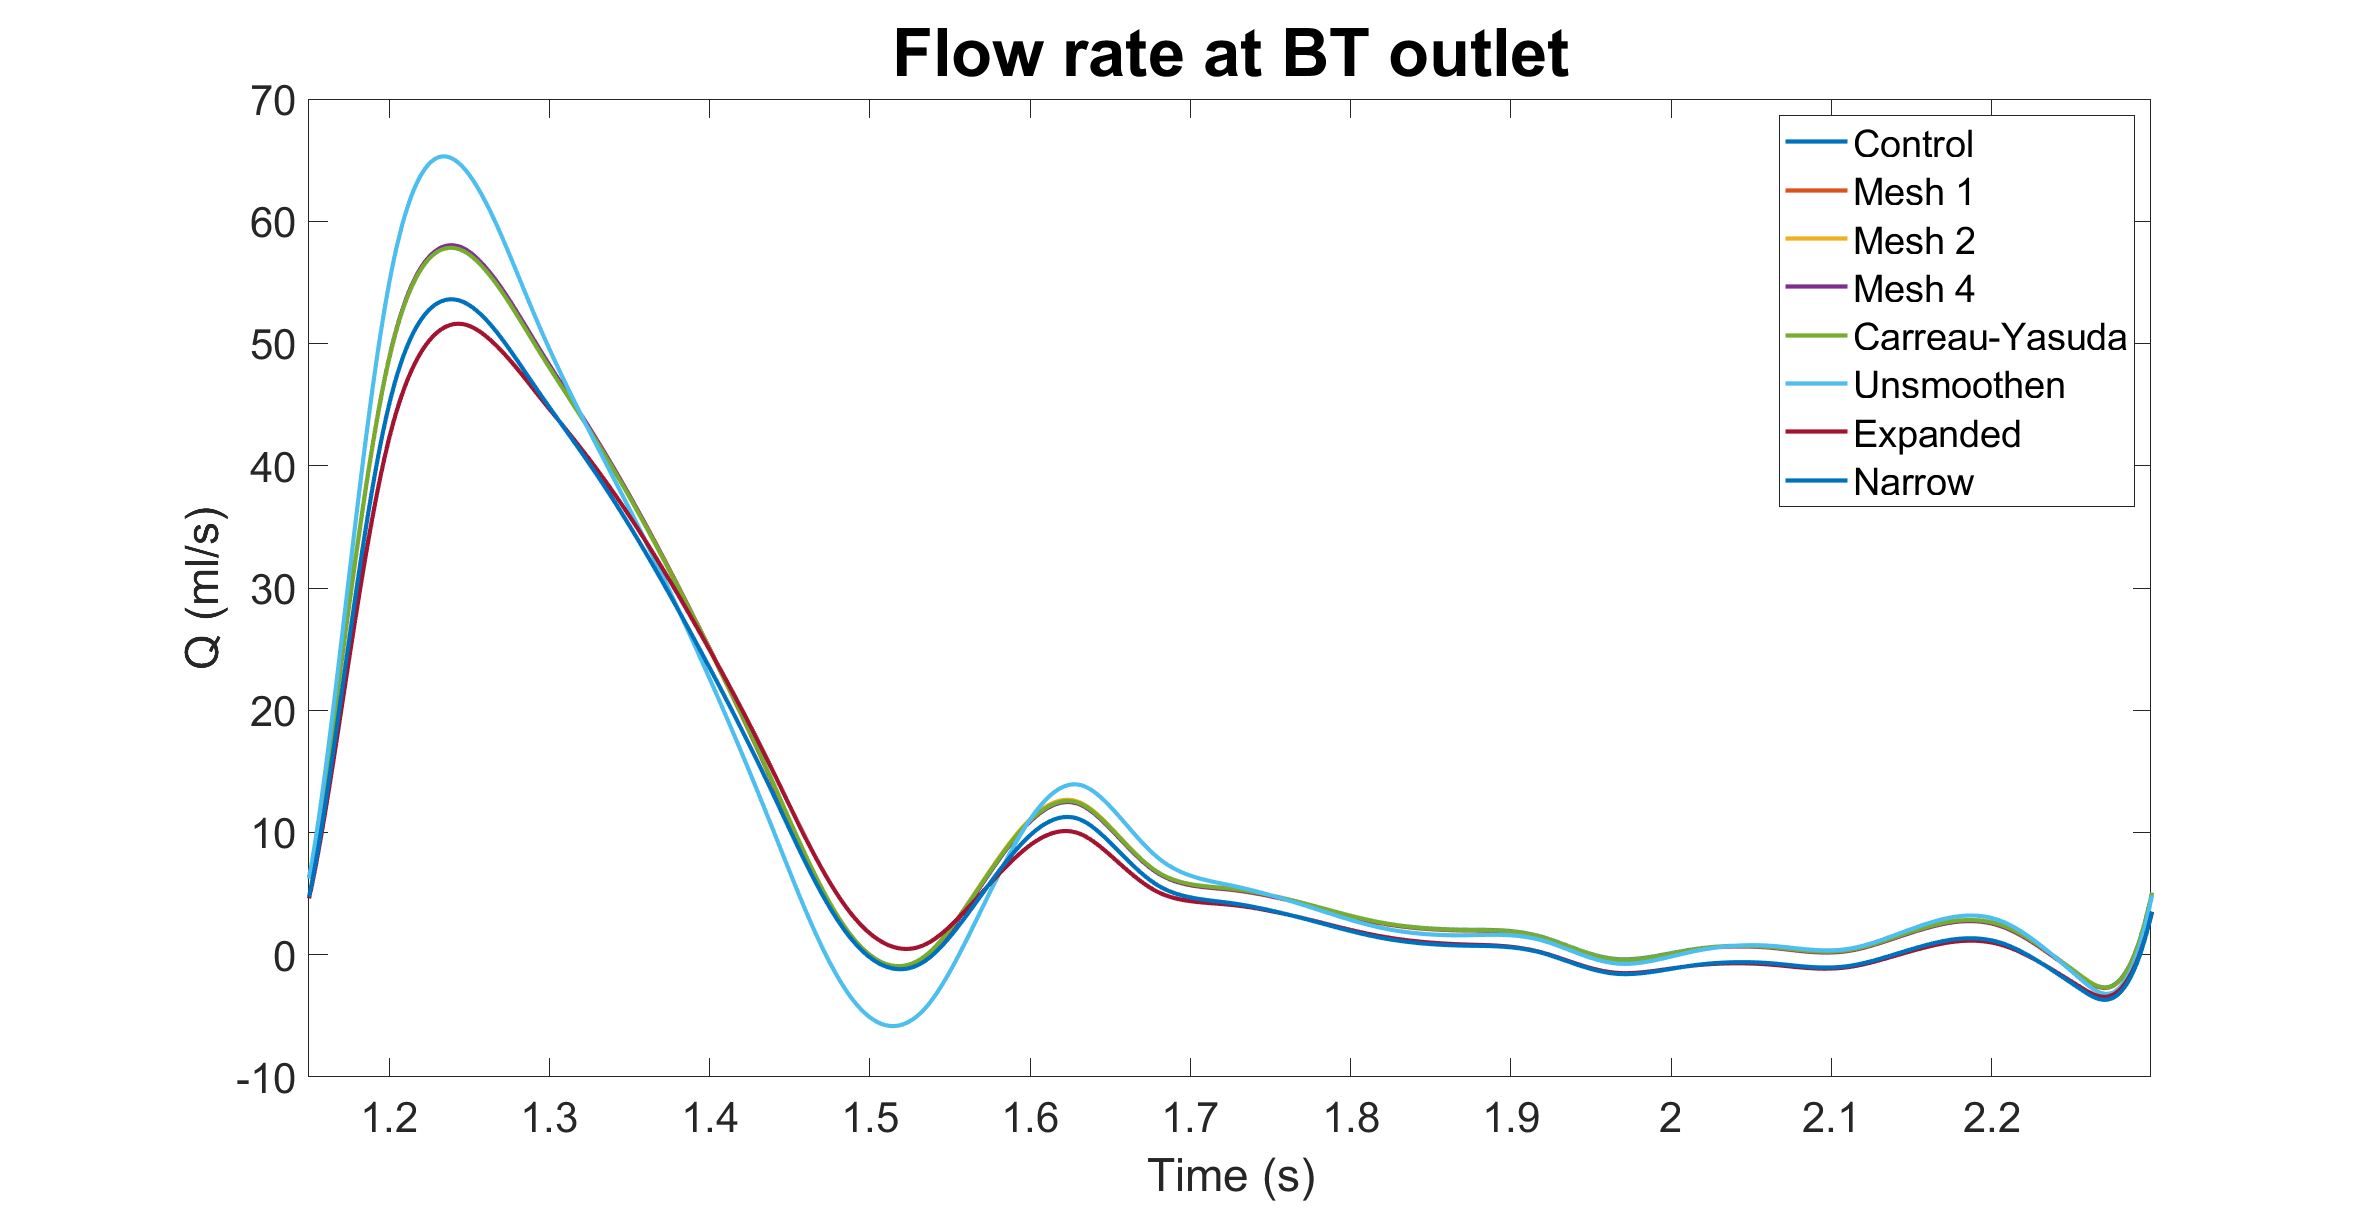
\includegraphics[width=\textwidth]{Figures/QBT.png}
     \end{subfigure}
     \hfill
     \begin{subfigure}[b]{0.49\textwidth}
         \centering
         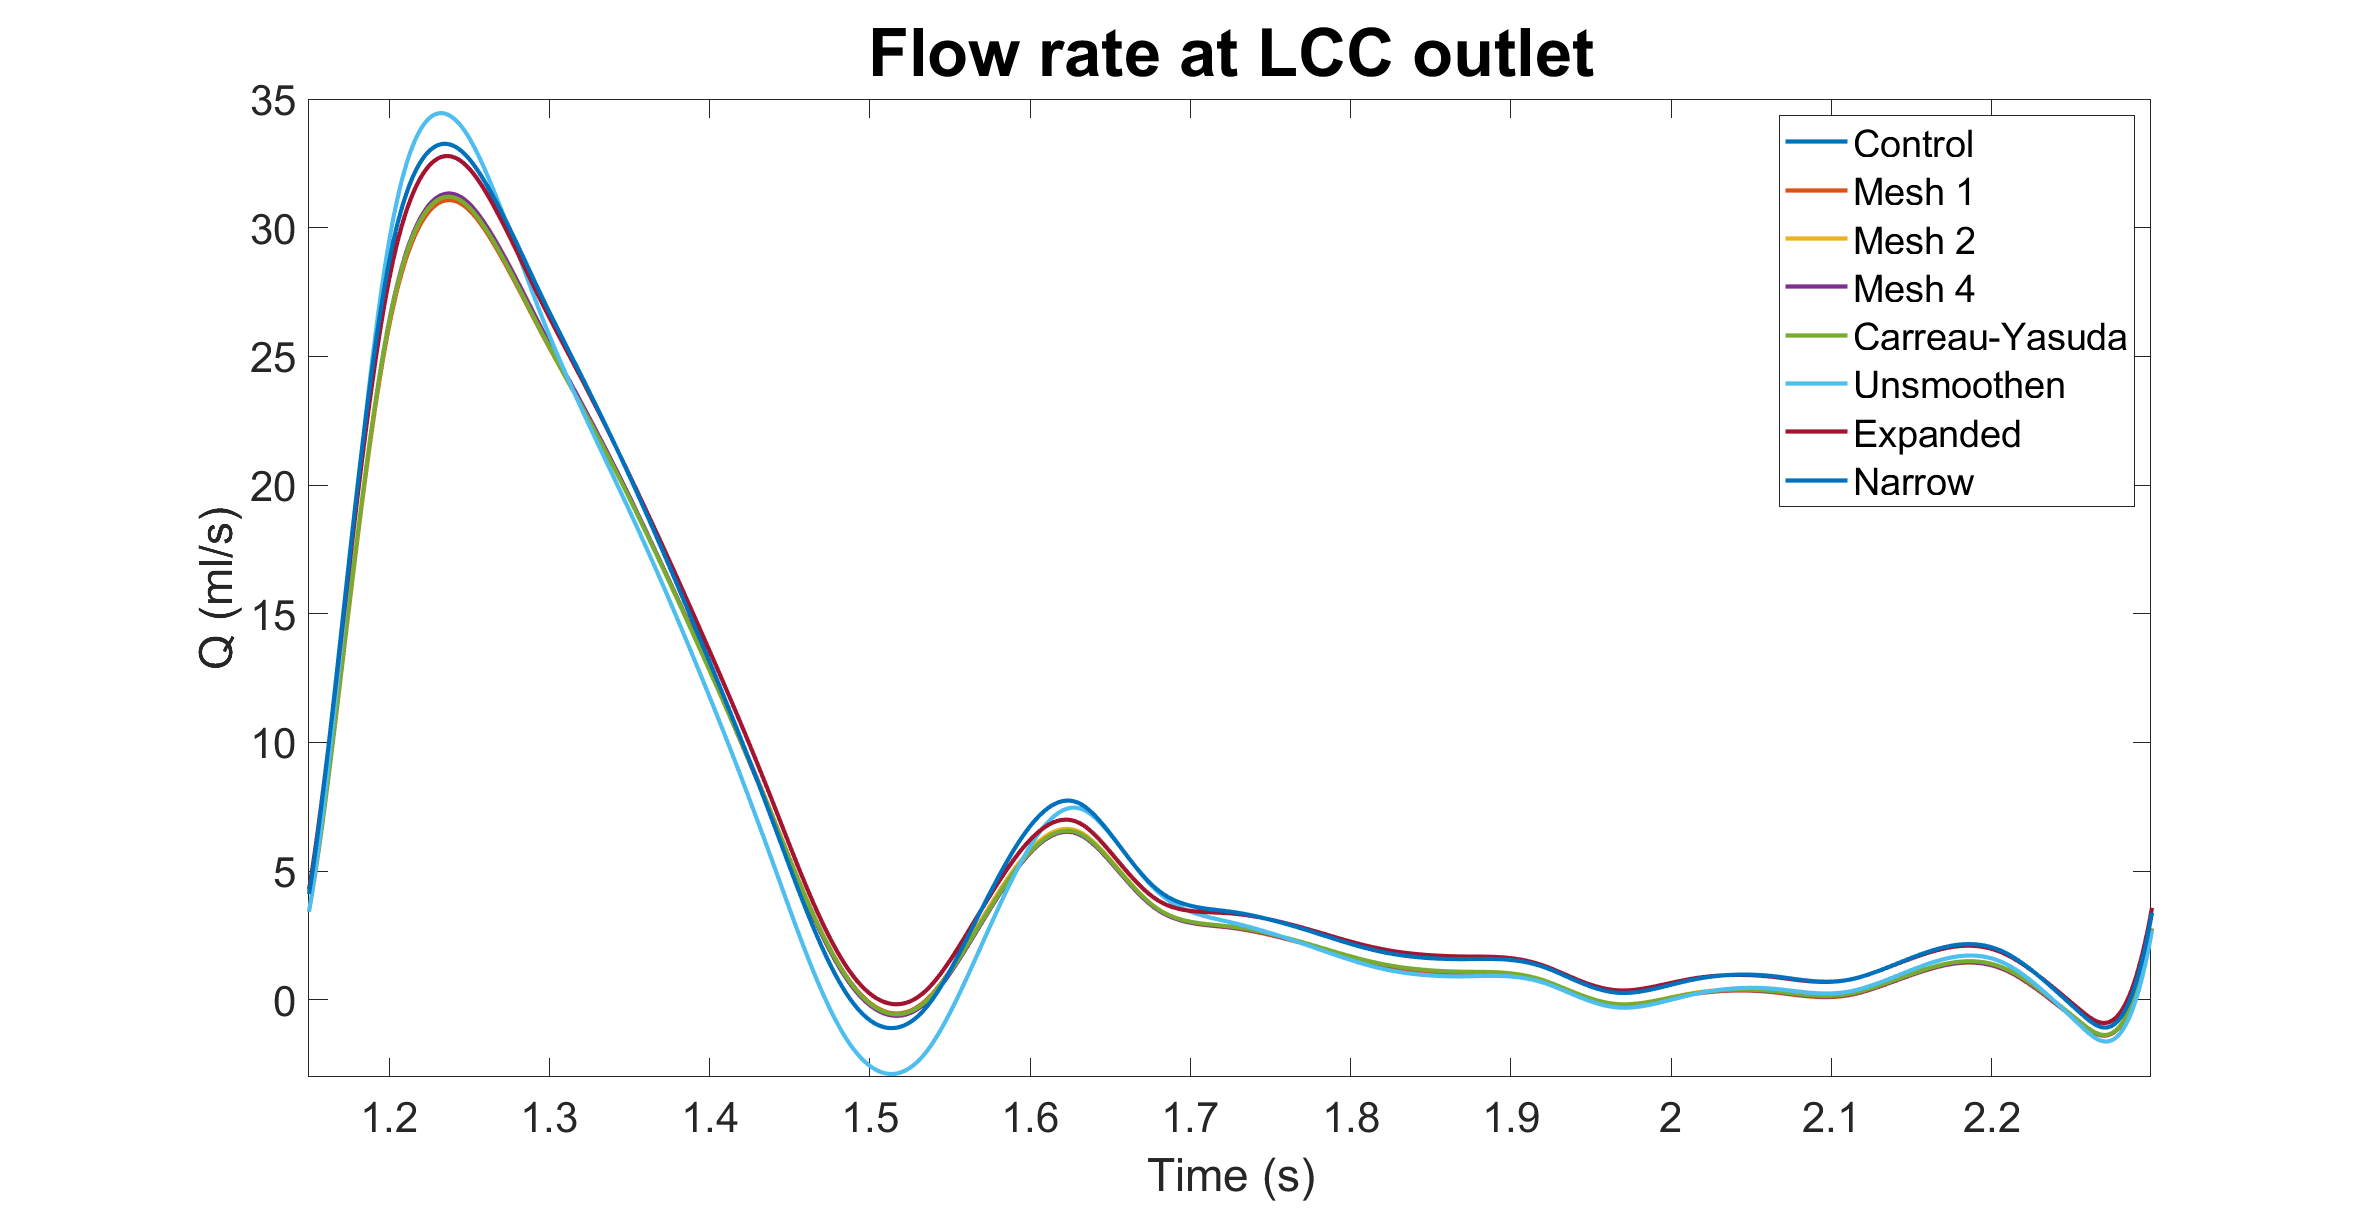
\includegraphics[width=\textwidth]{Figures/QLCC.png}
     \end{subfigure}
     \hfill
     \begin{subfigure}[b]{0.49\textwidth}
         \centering
         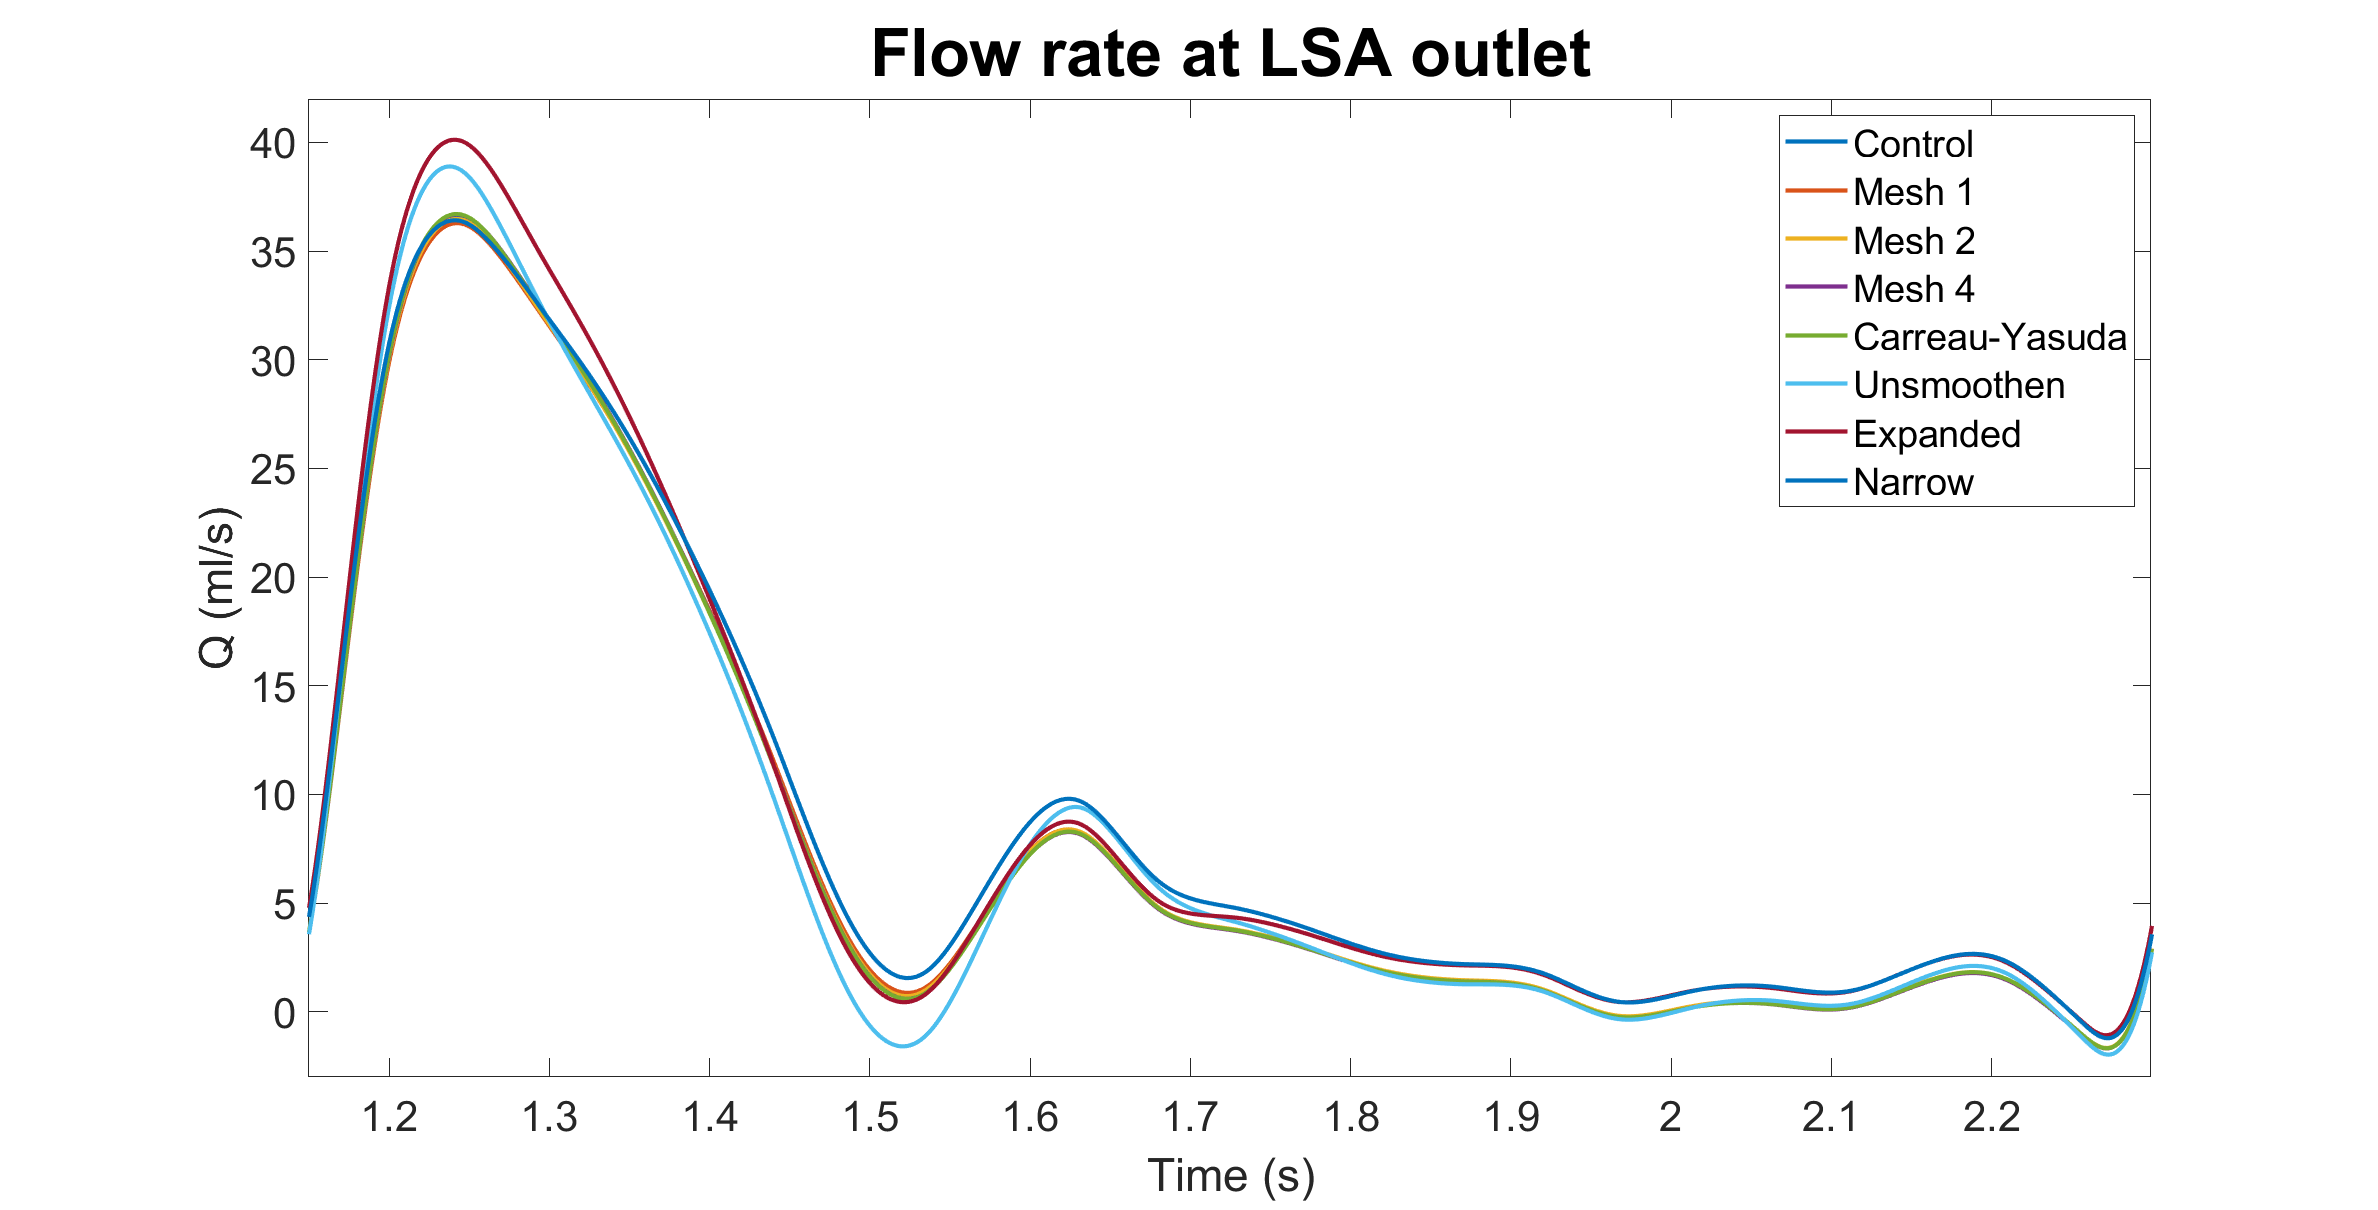
\includegraphics[width=\textwidth]{Figures/QLSA.png}
     \end{subfigure}
        \caption{The flow at the different outlets}
        \label{fig:flow}
\end{figure}

The most noticeable difference can be observed between the different segmentations of the patient aorta, where the mean difference of the flow at the outlet was 43.75\% followed by the image processing influence, where the difference was 34.05\%. The smallest difference was shown to be the influence of the viscosity model, as the difference across the outlets was smaller then 2\%. The influence of the mesh also showed to have very little effect on the outlet conditions where the flow rate differences were on average 2.64\%. \par

\begin{table}[ht!]
\resizebox{\textwidth}{!}{%
\begin{tabular}{l|ccccccccc}
 & \multicolumn{9}{c}{Mean absolute percentage error (\%)} \\
Model & $P_{AB}$ & $P_{BT}$ & $P_{LCC}$ & $P_{LSA}$ & $P_{in}$ & $Q_{AB}$ & $Q_{BT}$ & $Q_{LCC}$ & $Q_{LSA}$ \\ \hline
Mesh 1 & 0.05 & 0.07 & 0.11 & 0.12 & 0.07 & 9.11 & 10.28 & 18.69 & 3.49 \\
Mesh 2 & 0.07 & 0.07 & 0.07 & 0.09 & 0.07 & 4.69 & 5.78 & 3.22 & 9.32 \\
Mesh 4 & 0.05 & 0.05 & 0.06 & 0.05 & 0.05 & 4.59 & 8.20 & 6.05 & 1.69 \\
Carreau-Yasuda & 0.03 & 0.04 & 0.04 & 0.04 & 0.06 & 3.11 & 6.24 & 4.27 & 3.63 \\
Unsmoothened & 0.51 & 0.85 & 0.76 & 0.53 & 1.00 & 71.36 & 270.79 & 138.30 & 36.97 \\
Expanded & 0.32 & 0.39 & 0.34 & 0.50 & 0.53 & 16.38 & 234.40 & 245.78 & 152.72 \\
Narrow & 0.52 & 0.56 & 0.35 & 0.69 & 0.77 & 18.40 & 180.13 & 224.91 & 159.92
\end{tabular}%
}
\caption{The mean absolute percentage error at the different outlets}
\label{tab:pererr}
\end{table}

\section{Haemodynamic indices}
The results of time-averaged wall shear stress (TAWSS) can be seen on the Table \ref{tab:meanTAWSS}. On the Figures \ref{fig:TAWSScontrol}-\ref{fig:TAWSSGeo1}, the aorta was divided in sections along the centerline and at every section, a box plot of haemodynamic indices was plotted. The box plot shows the median of the values in the section with the red line, the $25^{th}$ and $75^{th}$ percentile of all the values and the maximum and the maximum the lines signify the maximum and minimum value. \par

\begin{table}[ht!]
\resizebox{\textwidth}{!}{%
\begin{tabular}{l|cccc}
 & \multicolumn{4}{c}{Mean TAWSS + SD at different locations (Pa)} \\
 & \multicolumn{1}{c|}{Ascending} & \multicolumn{1}{c|}{Arch} & \multicolumn{1}{c|}{Branches} & Descending \\ \hline
Control & \multicolumn{1}{c|}{0.996±0.630} & \multicolumn{1}{c|}{1.743±0.565} & \multicolumn{1}{c|}{1.979±0.893} & 1.152±0.388 \\
Mesh 1 & \multicolumn{1}{c|}{0.969±0.519} & \multicolumn{1}{c|}{1.714±0.543} & \multicolumn{1}{c|}{1.706±0.792} & 1.114±0.362 \\
Mesh 2 & \multicolumn{1}{c|}{0.986±0.562} & \multicolumn{1}{c|}{1.748±0.549} & \multicolumn{1}{c|}{1.832±0.829} & 1.154±0.390 \\
Mesh 4 & \multicolumn{1}{c|}{0.968±0.638} & \multicolumn{1}{c|}{1.708±0.556} & \multicolumn{1}{c|}{2.297±1.073} & 1.157±0.389 \\
CY & \multicolumn{1}{c|}{0.996±0.545} & \multicolumn{1}{c|}{1.633±0.478} & \multicolumn{1}{c|}{1.820±0.726} & 1.133±0.325 \\
Unsmoothened & \multicolumn{1}{c|}{1.357±0.798} & \multicolumn{1}{c|}{1.798±0.987} & \multicolumn{1}{c|}{2.468±1.522} & 1.757±0.852 \\
Expanded & \multicolumn{1}{c|}{0.949±0.554} & \multicolumn{1}{c|}{1.429±0.452} & \multicolumn{1}{c|}{1.431±0.588} & 1.012±0.291 \\
Narrow & \multicolumn{1}{c|}{1.151±0.719} & \multicolumn{1}{c|}{1.974±0.711} & \multicolumn{1}{c|}{2.598±1.592} & 1.302±0.514
\end{tabular}%
}
\caption{The mean TAWSS and the standard deviation (SD) of each model at different sections of the aorta}
\label{tab:meanTAWSS}
\end{table}

The most significant influence on the TAWSS can be seen on the model with the unsmoothened wall as a result of image processing where the median across all section is higher then the control mode and the spread of the values of TAWSS have a wider spread. \par

The different geometries yield different median and distribution of TAWSS, however the shape of the TAWSS along the centerline does not change and shows to be similar. The mesh does not have significant influence on the medians along the aorta with small changes in the distribution of TAWSS. Similar behaviour can be observed for the Carreau-Yasuda model. \par

The 3D plots of TAWSS are shown in the Appendix \ref{appendix1}.

\begin{figure}[ht!]
    \centering
    \includegraphics[width=\textwidth]{"Figures/Control TAWSS".png}
    \caption{Control Model TAWSS box plot along centerline}
    \label{fig:TAWSScontrol}
\end{figure}
\begin{figure}[ht!]
    \centering
    \includegraphics[width=\textwidth]{"Figures/Mesh1 TAWSS".png}
    \caption{Mesh 1 Model TAWSS box plot along centerline}
    \label{fig:TAWSSMesh1}
\end{figure}
\begin{figure}[ht!]
    \centering
    \includegraphics[width=\textwidth]{"Figures/Mesh2 TAWSS".png}
    \caption{Mesh 2 Model TAWSS box plot along centerline}
    \label{fig:TAWSSMesh2}
\end{figure}
\begin{figure}[ht!]
    \centering
    \includegraphics[width=\textwidth]{"Figures/Mesh4 TAWSS".png}
    \caption{Mesh 4 Model TAWSS box plot along centerline}
    \label{fig:TAWSSMesh4}
\end{figure}
\begin{figure}[ht!]
    \centering
    \includegraphics[width=\textwidth]{"Figures/Viscosity TAWSS".png}
    \caption{Carreau-Yasuda Model TAWSS box plot along centerline}
    \label{fig:TAWSSVis}
\end{figure}
\begin{figure}[ht!]
    \centering
    \includegraphics[width=\textwidth]{"Figures/Img TAWSS".png}
    \caption{Unsmoothened Model TAWSS box plot along centerline}
    \label{fig:TAWSSImg}
\end{figure}
\begin{figure}[ht!]
    \centering
    \includegraphics[width=\textwidth]{"Figures/Expanded TAWSS".png}
    \caption{Expanded lumen model TAWSS box plot along centerline}
    \label{fig:TAWSSGeo1}
\end{figure}
\begin{figure}[ht!]
    \centering
    \includegraphics[width=\textwidth]{"Figures/Narrow TAWSS".png}
    \caption{Narrow lumen model TAWSS box plot along centerline}
    \label{fig:TAWSSGeo2}
\end{figure}

